
\documentclass{article}
\usepackage{tikz}
\begin{document}
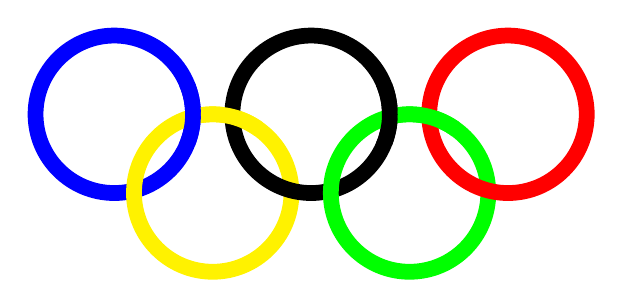
\begin{tikzpicture}
    \draw [line width=0.2cm, blue] (-2.5, 0) circle (1cm);
    \draw [line width=0.2cm, yellow] (-1.25, -1) circle (1cm);
    \draw [line width=0.2cm] (0, 0) circle (1cm);
    \draw [line width=0.2cm, green] (1.25, -1) circle (1cm);
    \draw [line width=0.2cm, red] (2.5, 0) circle (1cm);
    \begin{scope}
        \clip (-1.5, 0) circle (0.4);
        \draw [line width=0.2cm, blue] (-2.5, 0) circle (1cm);
    \end{scope}
    \begin{scope}
        \clip (-1, 0) circle (0.4);
        \draw [line width=0.2cm, yellow] (-1.25, -1) circle (1cm);
    \end{scope}
    \begin{scope}
        \clip (1, 0) circle (0.4);
        \draw [line width=0.2cm] (0, 0) circle (1cm);
    \end{scope}
    \begin{scope}
        \clip (1.5, 0) circle (0.4);
        \draw [line width=0.2cm, green] (1.25, -1) circle (1cm);
    \end{scope}
\end{tikzpicture}
\end{document}

